\documentclass{beamer}

\usetheme{uhh}
\showtotalframenumber
\showuhhlogoeachframe
\showsections

\usepackage{booktabs}

\usepackage{amsmath}
\usepackage{graphicx}
\usepackage{color}
\DeclareMathOperator*{\argmin}{arg\,min}

\usepackage{listings}
\lstset{
  language=python
  }


\title{Inducing Interpretable Word Senses for WSD and Enrichment of Lexical Resources}

%\institute[University of Hamburg] 
%{
%  Faculty of Mathematics, Informatics, and Natural Sciences \\
%  Department of Informatics\\
%  Language Technology Group
%}


\author{Alexander Panchenko} % \\University of Hamburg, Germany}
\date[11.02.2018]{Jan 11, 2018}


\AtBeginSection[]
{
   %%%%% section title
   % This is how it would look like in Beamer:
   % \begin{frame}
   %     \frametitle{Overview}
   %     \tableofcontents[sections={2-3},currentsection,sectionstyle=show/hide,subsectionstyle=hide]
   % \end{frame}
  \begin{frame}[plain]
  \begin{tikzpicture}[overlay]
    \relax%
    \fill[blueuhh,opacity=1] (-10,-10)
    rectangle(\the\paperwidth,\the\paperheight);
  \end{tikzpicture}
   \begin{tikzpicture}[overlay]
    \relax%
    \fill[white,opacity=1] (-5,-1.2)
    rectangle(\the\paperwidth,0.5) node[pos=0.5,black]{\LARGE\insertsectionhead};
  \end{tikzpicture}
  \end{frame}

  %%%% add subsection to show navigation dots
  \subsection{}
}

\begin{document}

\maketitle


\section{Overview}

\begin{frame}
  \frametitle{Overview}

  \begin{itemize}
		\item \textbf{Inducing word sense representations}:
		\begin{itemize}
		\item word sense embeddings via retrofitting \cite{pelevina-EtAl:2016:RepL4NLP,remus:2018};
		\item sparse sense representations \cite{panchenko-EtAl:2017:EACLlong};
		\item inducing synsets~\cite{ustalov-panchenko-biemann:2017:Long}
		\item sense semantic classes \cite{panchenko:2018:SemanticClasses} 
		\end{itemize}
		
	\pause 
	\vspace{1em}
	\item \textbf{Making induced senses interpretable} \cite{panchenko-EtAl:2017:EMNLP2017Demos,panchenko-EtAl:2017:EACLlong}
	
	\pause
	\vspace{1em}
	\item \textbf{Linking induced word senses to lexical resources}~\cite{faralli2016linked,panchenko-EtAl:2017:SENSE2017,biemann2018framework}	
			
\end{itemize}
	
\end{frame}

\section{Inducing word sense representations}


\subsection{Related work}
\begin{frame}[fragile]
\frametitle{Related work}
\begin{center}
 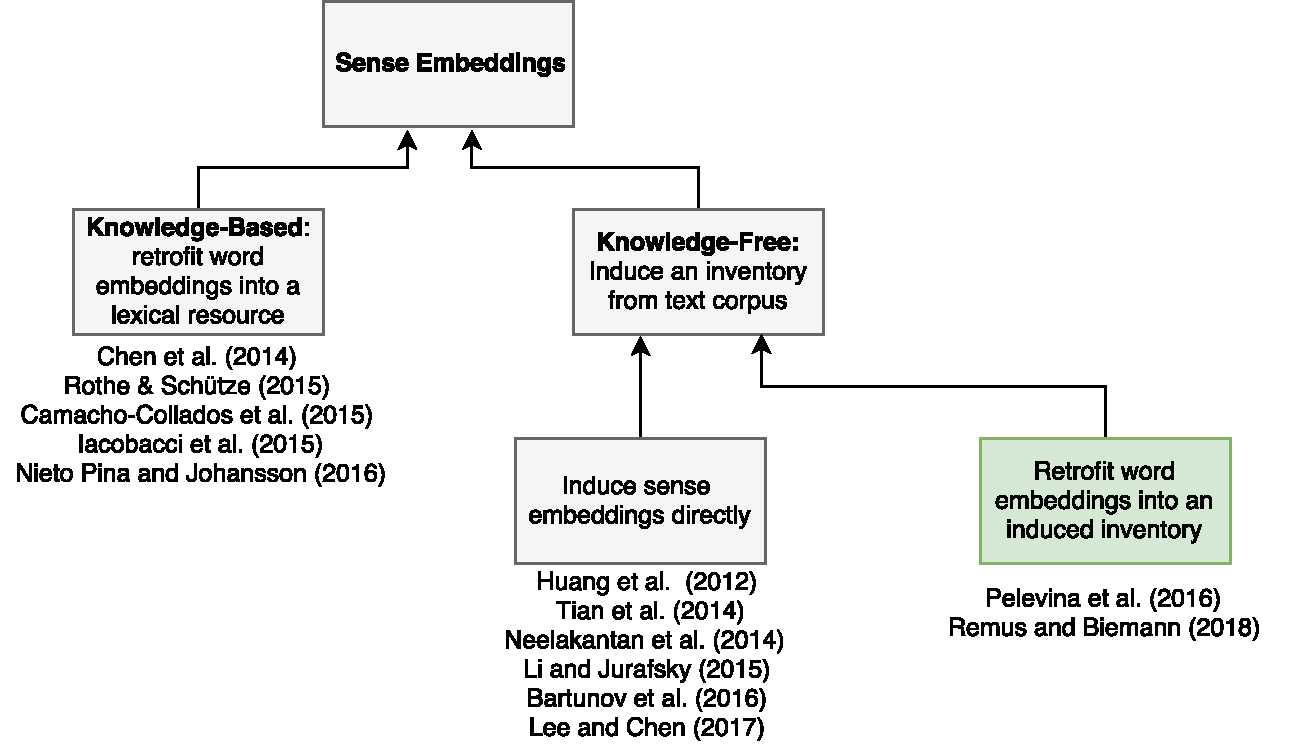
\includegraphics[height=0.56\textwidth]{sense_embeddings}
 \end{center}
\end{frame}


\begin{frame}
\frametitle{Related work: knowledge-based}
\begin{itemize}
	\item \textbf{AutoExtend}~\cite{rothe-schutze:2015:ACL-IJCNLP}
\end{itemize}
\begin{center}
 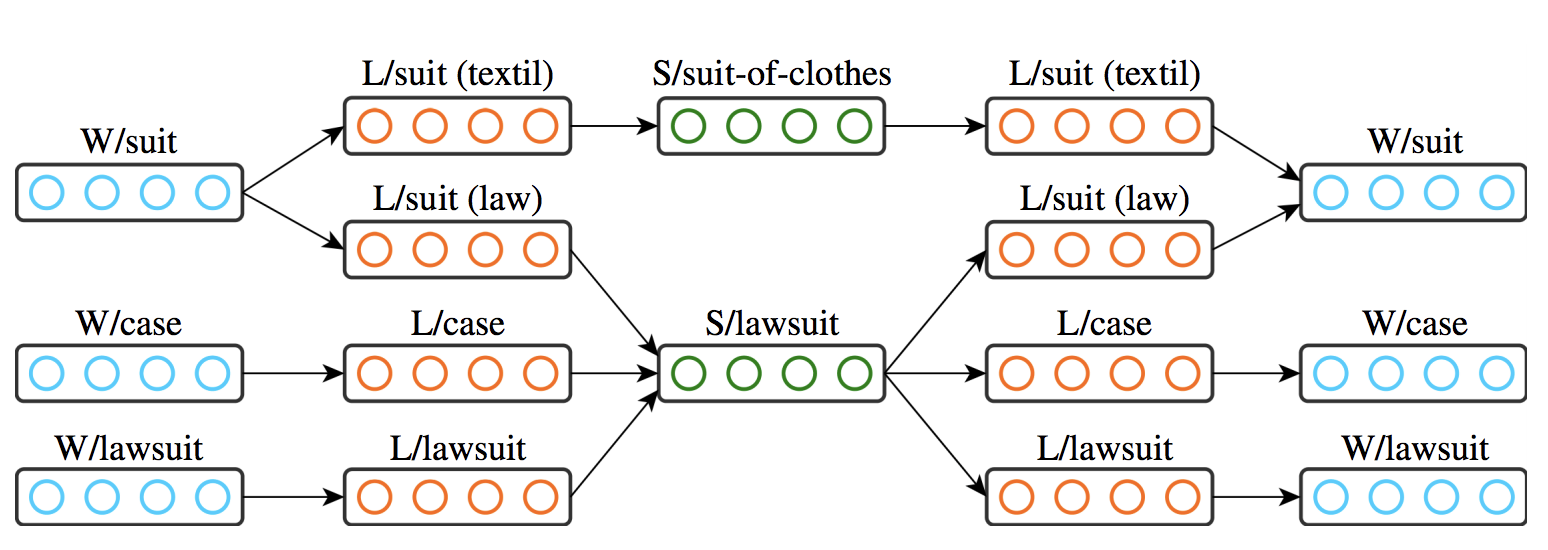
\includegraphics[width=1.0\textwidth]{autoextend}
 \end{center}

{\footnotesize
 * image is reproduced from the original paper
}

\end{frame}

\begin{frame}{Related work: knowledge-free}

\begin{itemize}
\item \textbf{Adagram}~\cite{bartunov2016breaking}
\item Multiple vector representations $\theta$ for each word:
%\item An bayesian extension of the Skip-gram model:
 $$p(Y,Z,\mathbf{\beta}|X,\alpha,\theta) = \prod_{w=1}^{V} \prod_{k=1}^{\infty} p(\beta_{wk}|\alpha) \prod_{i=1}^N [p(z_i|x_i,\mathbf{\beta}) \prod_{j=1}^C p(y_{ij}|z_i,x_i,\theta)],$$ 
\begin{itemize}

\pause 

\item $\alpha$ -- a meta-parameter controlling number of senses;
\item $z_i$ -- a hidden variable: a sense index in context; 
\item $p(\beta_{wk}|\alpha)$ -- probability of the $k$-th sense of the word $w$;
\item $p(z_i|x_i,\mathbf{\beta})$ -- probability of observing word $x_i$ in the sense $z_i$;
\item $\prod_{j=1}^C p(y_{ij}|z_i,x_i,\theta)$ -- probability of the context $C$.
\end{itemize}

\pause 
\item \alert{\textbf{See also}}: [Neelakantan et al., 2014] and [Li and Jurafsky, 2015]

\end{itemize}
	
\end{frame}


\begin{frame}{Related work: word sense induction}

\begin{itemize}
	\item Word sense induction (WSI) based on \alert{\textbf{graph clustering}}:  
	\begin{itemize}
	\item $ $ [Lin, 1998]
	\item $ $ [Pantel and Lin, 2002]
	\item $ $ [Widdows and Dorow, 2002]
	\item $ $ \textbf{Chinese Whispers [Biemann, 2006]}
	\item $ $ [Hope and Keller, 2013]
	\end{itemize}
	
	%\item ...we extend this line of work.
\end{itemize}
	

\end{frame}



\begin{frame}[fragile]
\frametitle{Related work: Chinese Whispers\#1}
\begin{center}
 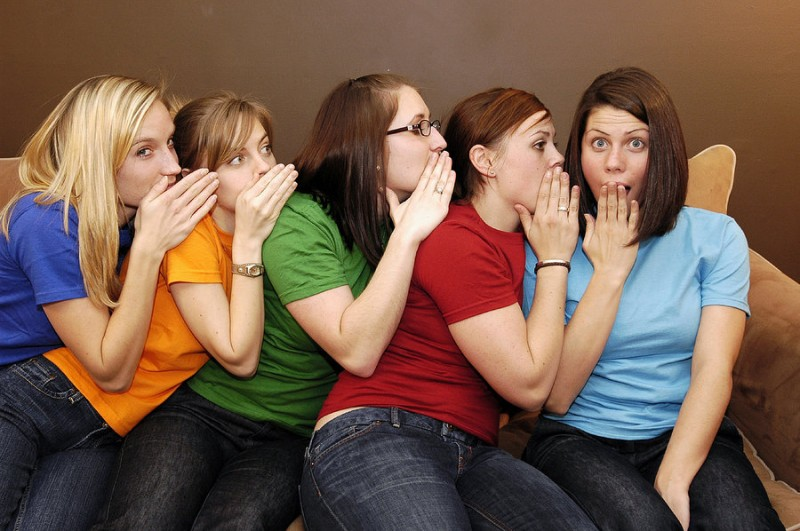
\includegraphics[height=0.5\textwidth]{cw}
 
  {\tiny * source of the image: \url{http://ic.pics.livejournal.com/blagin_anton/33716210/2701748/2701748_800.jpg}}
 \end{center}
\end{frame}



\begin{frame}[fragile]
\frametitle{Related work: Chinese Whispers\#2}
\begin{center}
 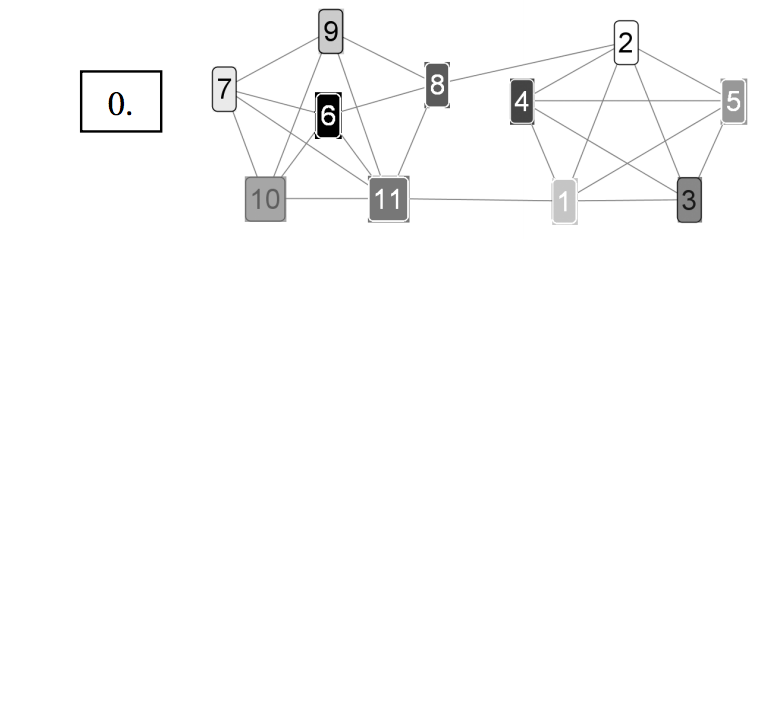
\includegraphics[height=0.59\textwidth]{cw2-1}
 
  %{\tiny * source of the image: [Biemann, 2006]}
 \end{center}
\end{frame}


\begin{frame}[fragile]
\frametitle{Related work: Chinese Whispers\#2}
\begin{center}
 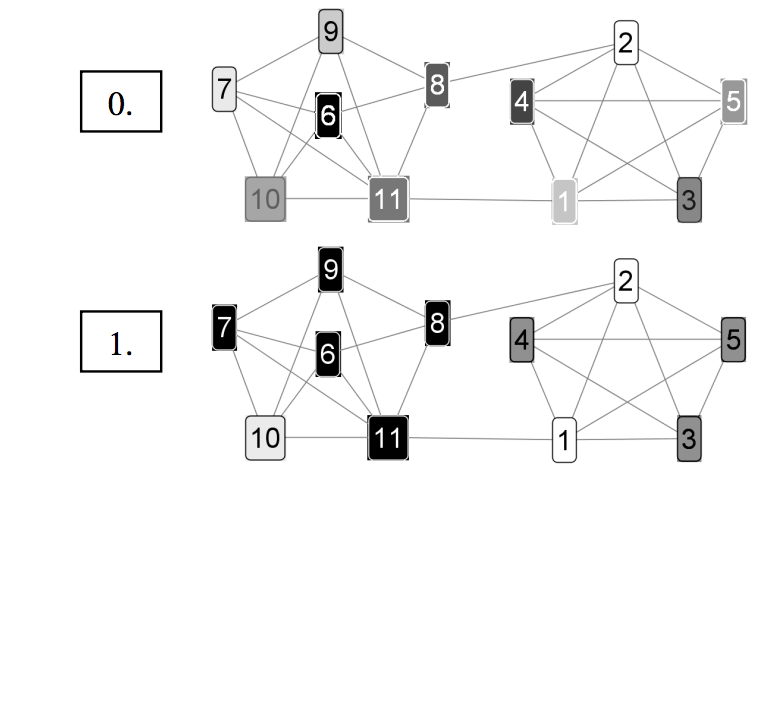
\includegraphics[height=0.59\textwidth]{cw2-2}
 
  %{\tiny * source of the image: [Biemann, 2006]}
 \end{center}
\end{frame}

\begin{frame}[fragile]
\frametitle{Related work: Chinese Whispers\#2}
\begin{center}
 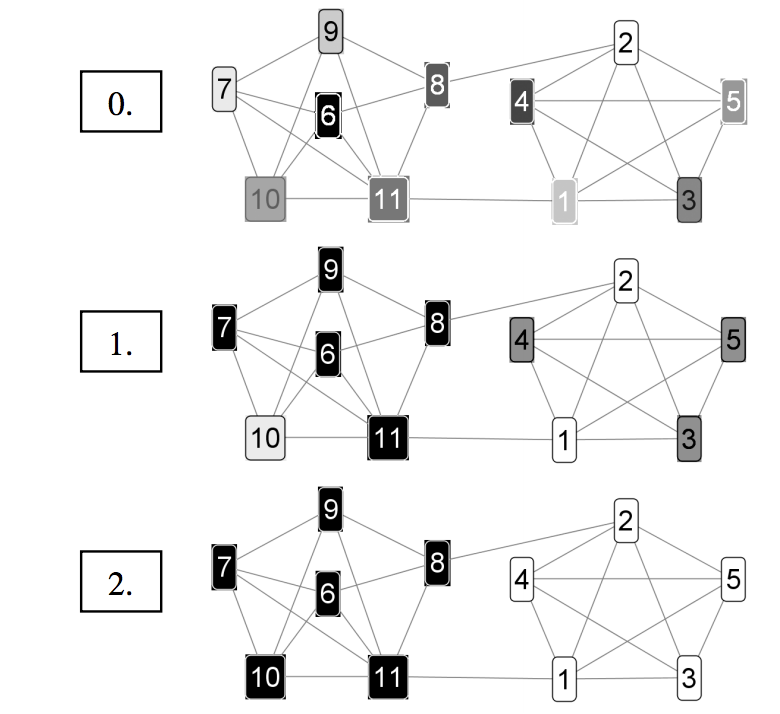
\includegraphics[height=0.59\textwidth]{cw2}
 
  %{\tiny * source of the image: [Biemann, 2006]}
 \end{center}
\end{frame}



\begin{frame}{Sense embeddings using retrofitting}
	
	%\begin{itemize} 
	 {\footnotesize RepL4NLP@ACL'16 \cite{pelevina-EtAl:2016:RepL4NLP}, LREC'18 \cite{remus:2018}}
	%\end{itemize}
	
	\begin{block}{Prior methods:}
		\vspace{0.25cm}

	\begin{itemize}	
	\item Induce inventory by \alert{clustering of word instances} %(Li and Jurafsky, 2015)
	\item Use \alert{existing} sense inventories %(Rothe and Sch\"{u}tze, 2015)	
	\end{itemize}
\end{block}


	\begin{block}{Our method:}
		\vspace{0.25cm}

	\begin{itemize}	
	\item \textbf{Input:} word embeddings
	\item \textbf{Output:} word sense embeddings
	\item \textbf{Word sense induction} by \alert{clustering of word ego-networks}
	%\item \textbf{Word sense disambiguation} based on the induced sense representations

	\end{itemize}
\end{block}


\end{frame}

\begin{frame}{Sense embeddings using retrofitting}
\begin{itemize}
\item From word embeddings to sense embeddings
\end{itemize}
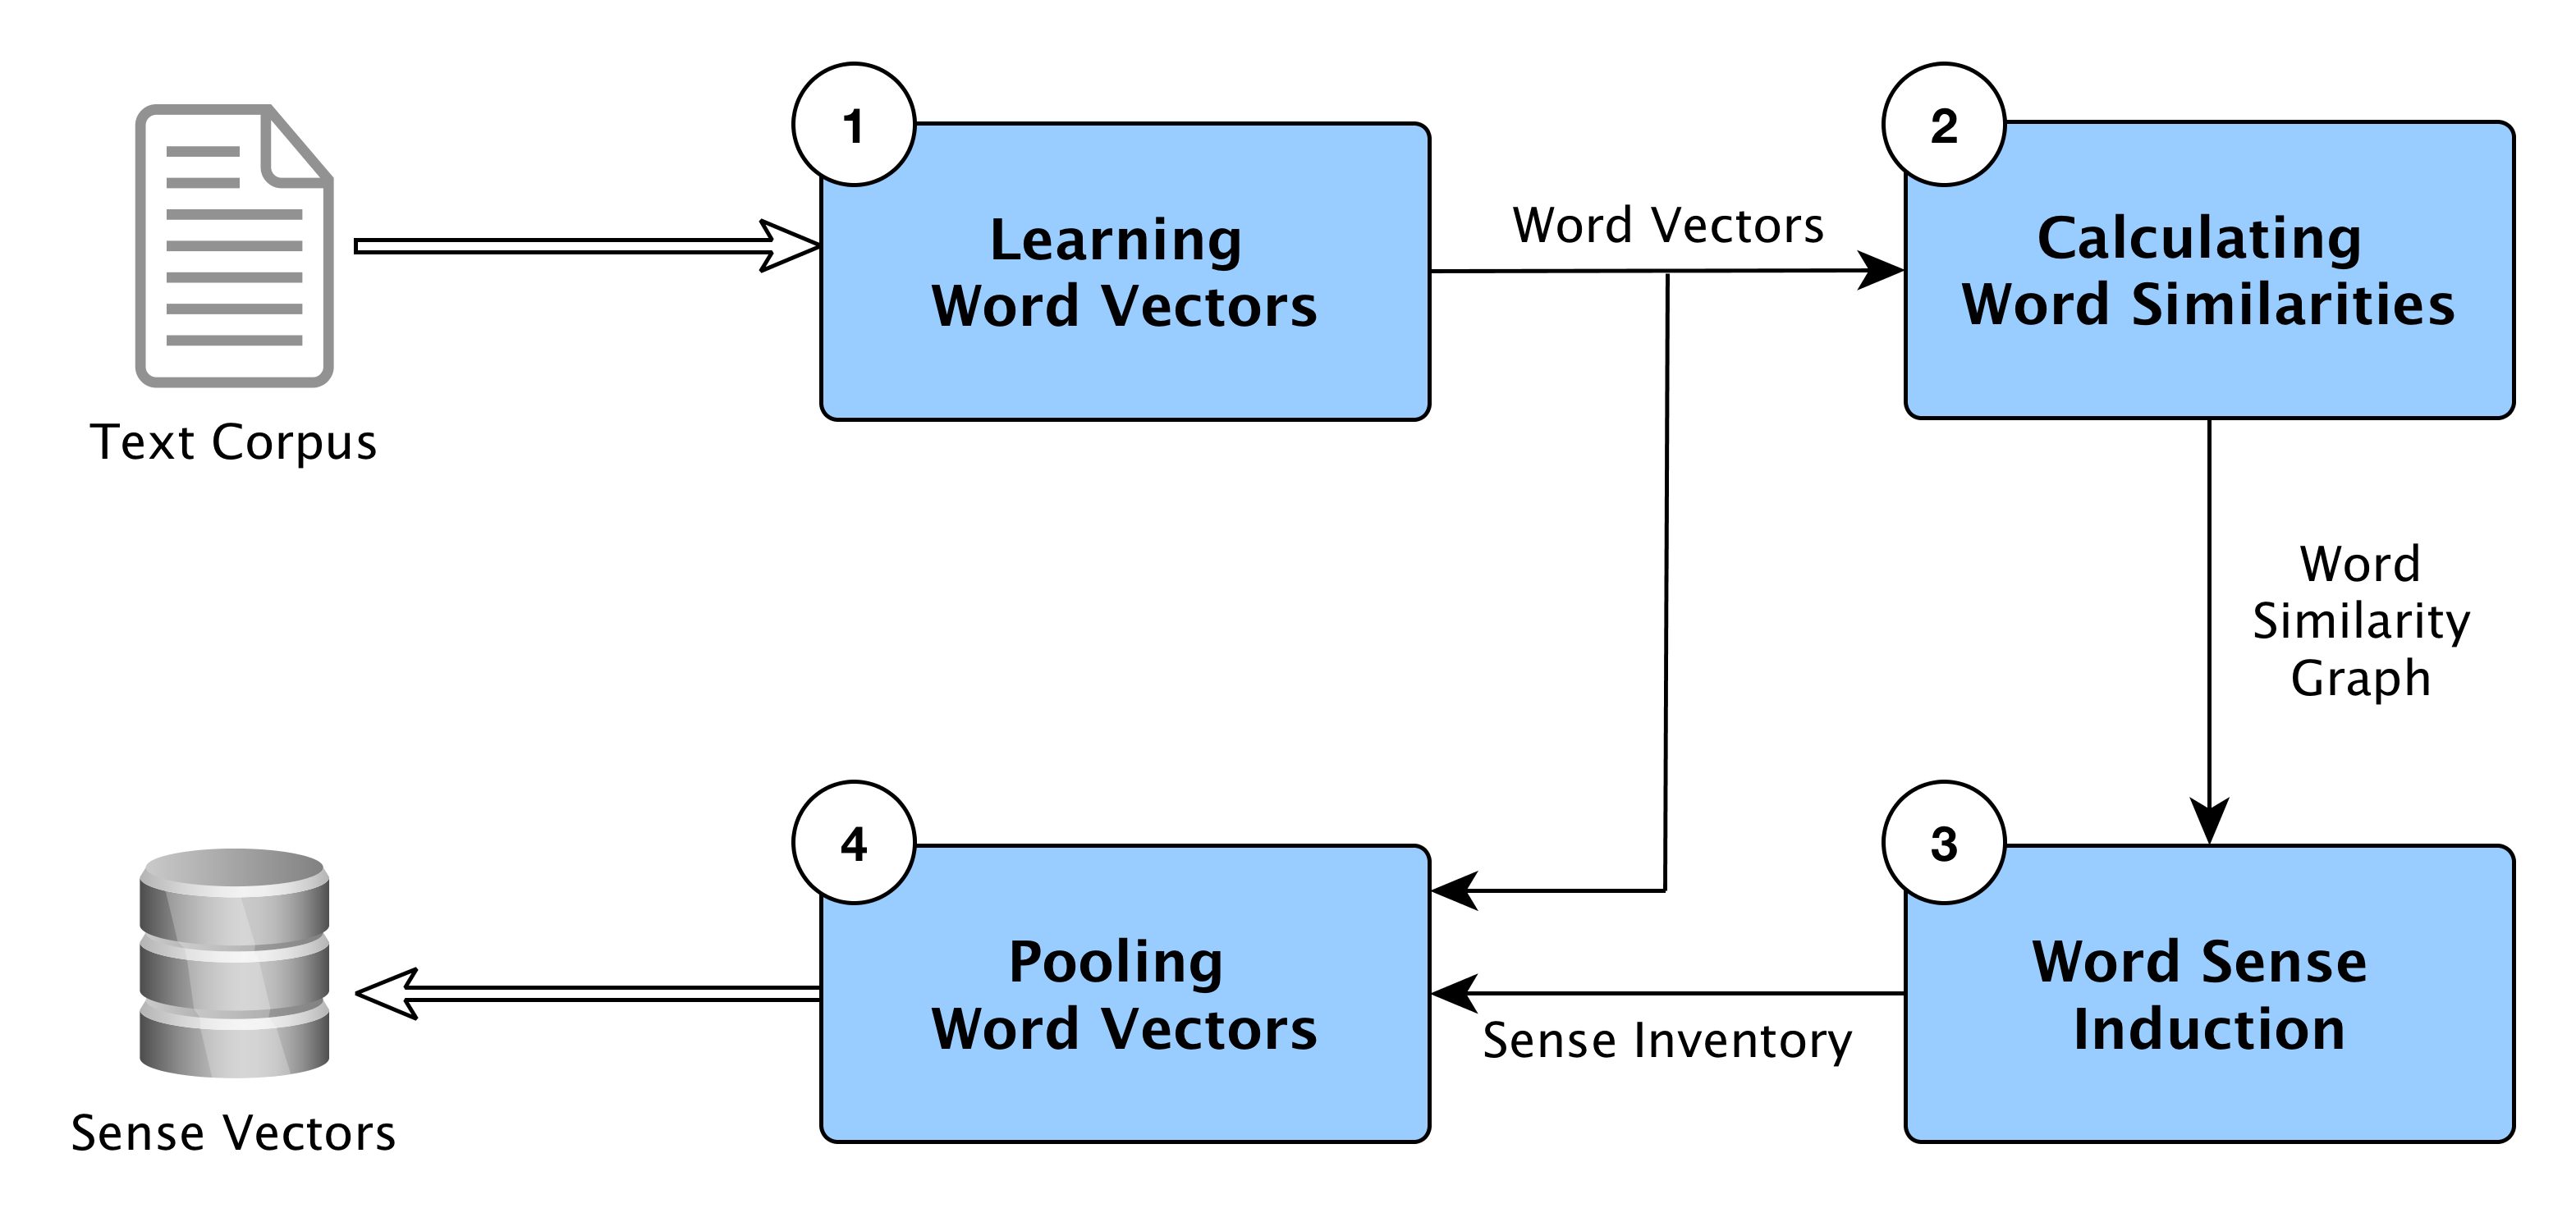
\includegraphics[width=\textwidth]{pipeline}

\end{frame}



\begin{frame}{Sense embeddings using retrofitting}

\begin{itemize}
\item Word sense induction using  ego-network clustering
\end{itemize} 
	
\centering
\begin{figure}
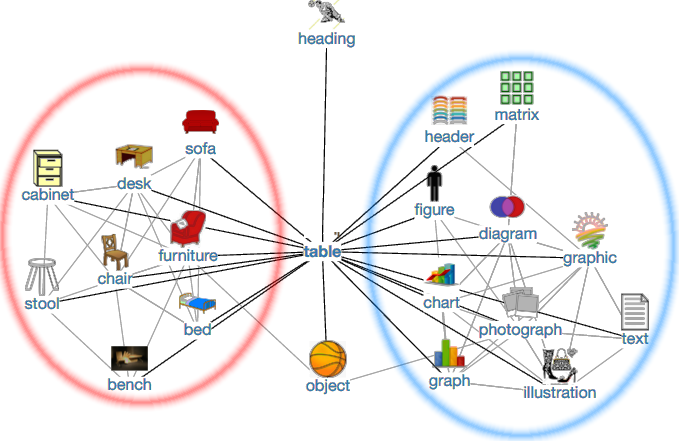
\includegraphics[width=0.75\textwidth]{table}
\end{figure}

\end{frame}


\begin{frame}{Sense embeddings using retrofitting}

\begin{itemize}
	\item Neighbours of Word and Sense Vectors
\end{itemize}


%\begin{table}
%
%\footnotesize
%\centering

\begin{tabular}{l|p{9cm}}
\bf Vector & \bf {Nearest Neighbors} \\ \toprule
 table & $ $ \alert{tray}, bottom, diagram, \alert{bucket}, brackets, stack, \alert{basket}, list, parenthesis, \alert{cup}, \alert{trays}, \alert{pile}, \alert{playfield}, bracket, \alert{pot}, drop-down, \alert{cue}, \alert{plate} \\ \midrule
 \pause
  table\#0 & $ $ leftmost\#0,  column\#1,  randomly\#0,  tableau\#1, top-left\#0, indent\#1,  bracket\#3,  pointer\#0,  footer\#1, cursor\#1, diagram\#0, grid\#0 \\ \midrule
   table\#1 & $ $ \alert{pile\#1,  stool\#1,  tray\#0,  basket\#0,  bowl\#1,  bucket\#0,  box\#0,  cage\#0,  saucer\#3,      mirror\#1,  birdcage\#0,  hole\#0,  pan\#1,  lid\#0}  \\ 
\end{tabular}
%\end{table}
%
%\begin{itemize}
%	\item Neighbours of the word ``table" and its senses produced by our method.
%	\item The neighbours of the initial vector belong to \textbf{both senses}.
%	\item The neighbours of the sense vectors are \textbf{sense-specific}.   
%\end{itemize}

	

\end{frame}




\begin{frame}{Sense embeddings using retrofitting}
	
	\begin{block}{Word Sense Disambiguation}
	
	\begin{enumerate} 
	\item \textbf{\alert{Context extraction}}: use context words around the target word
	\item \textbf{\alert{Context filtering}}: based on context word's relevance for disambiguation
	
	\item \textbf{\alert{Sense choice in context}}: maximise similarity between a context vector and a sense vector
	
	\end{enumerate}
	\end{block}

\end{frame}


\begin{frame}{Sense embeddings using retrofitting}
\vspace{-3em}
\begin{center}
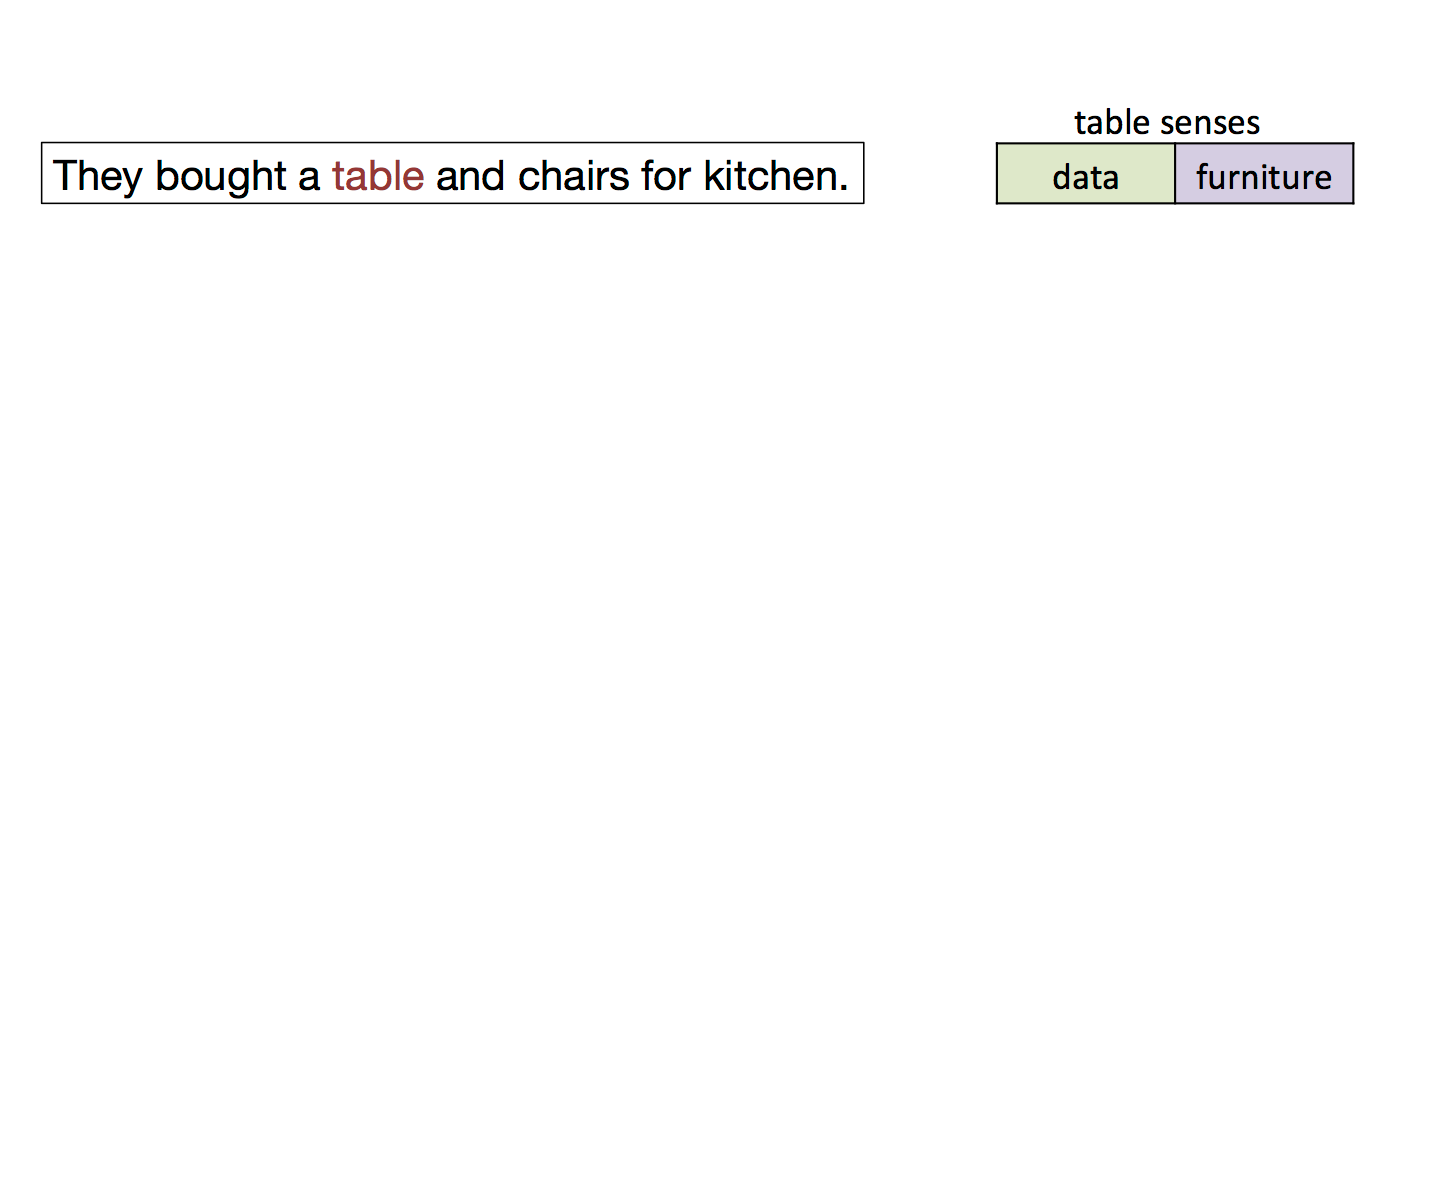
\includegraphics[width=0.82\textwidth]{wsd-1}
\end{center}	
\end{frame}



\begin{frame}{Sense embeddings using retrofitting}
\vspace{-3em}
\begin{center}
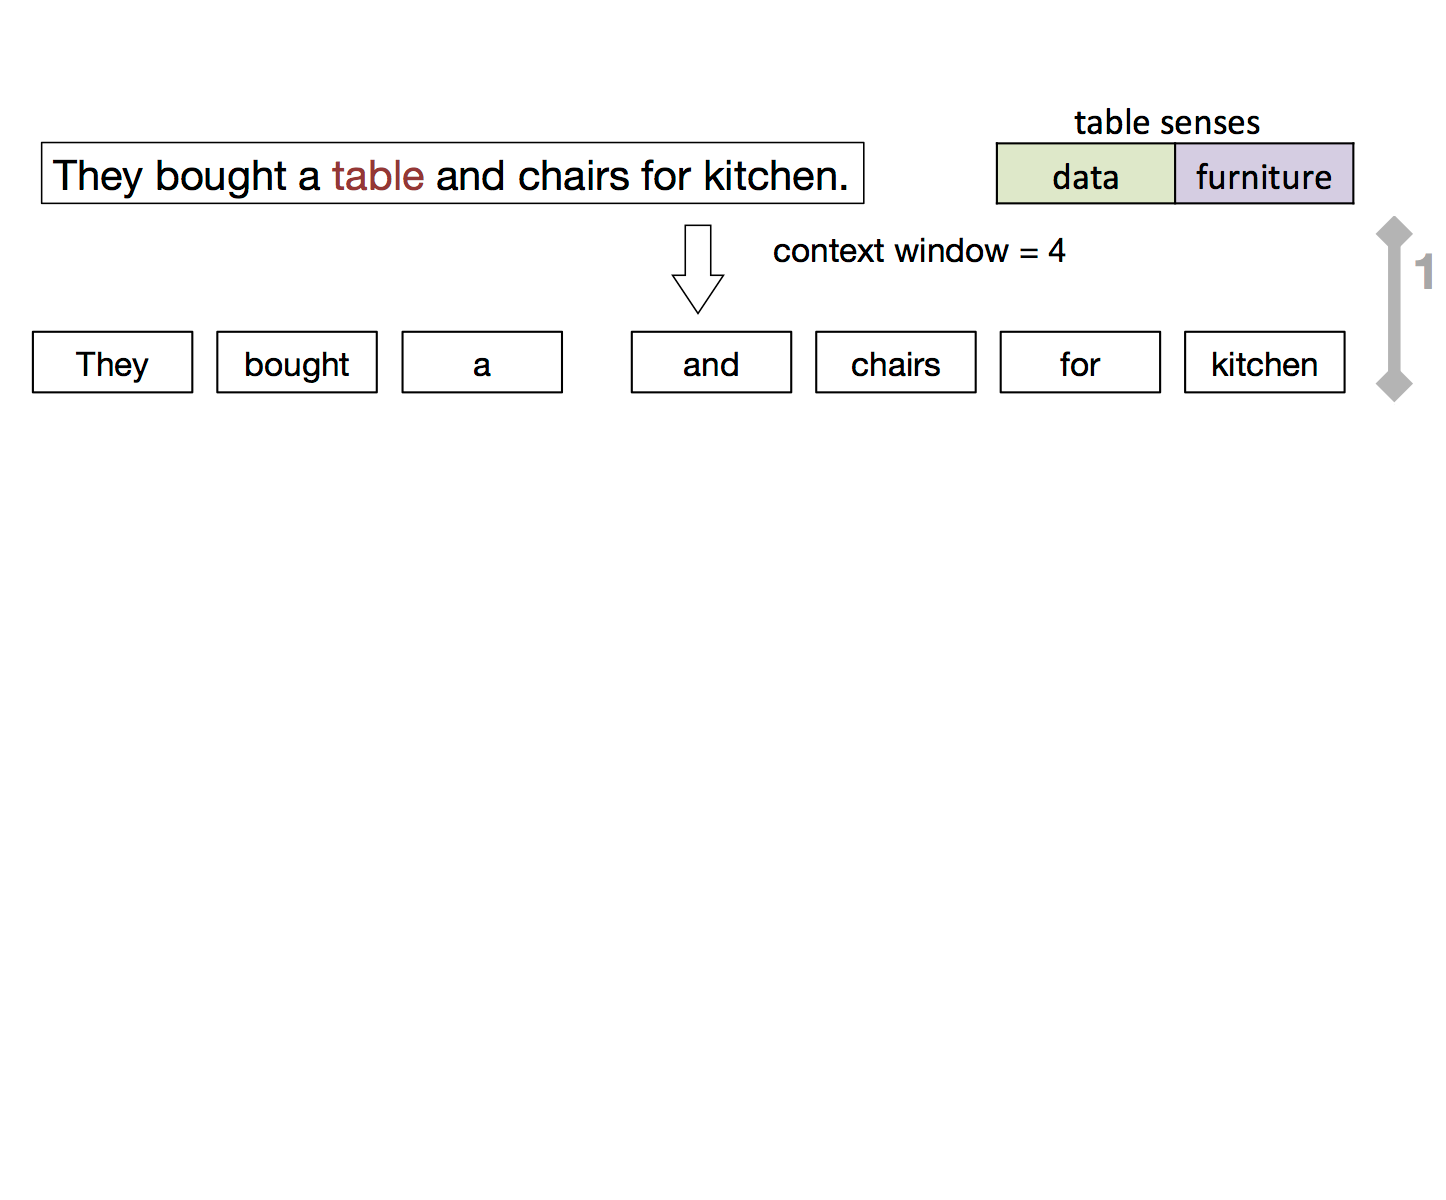
\includegraphics[width=0.82\textwidth]{wsd-2}
\end{center}	
\end{frame}



\begin{frame}{Sense embeddings using retrofitting}
\vspace{-3em}
\begin{center}
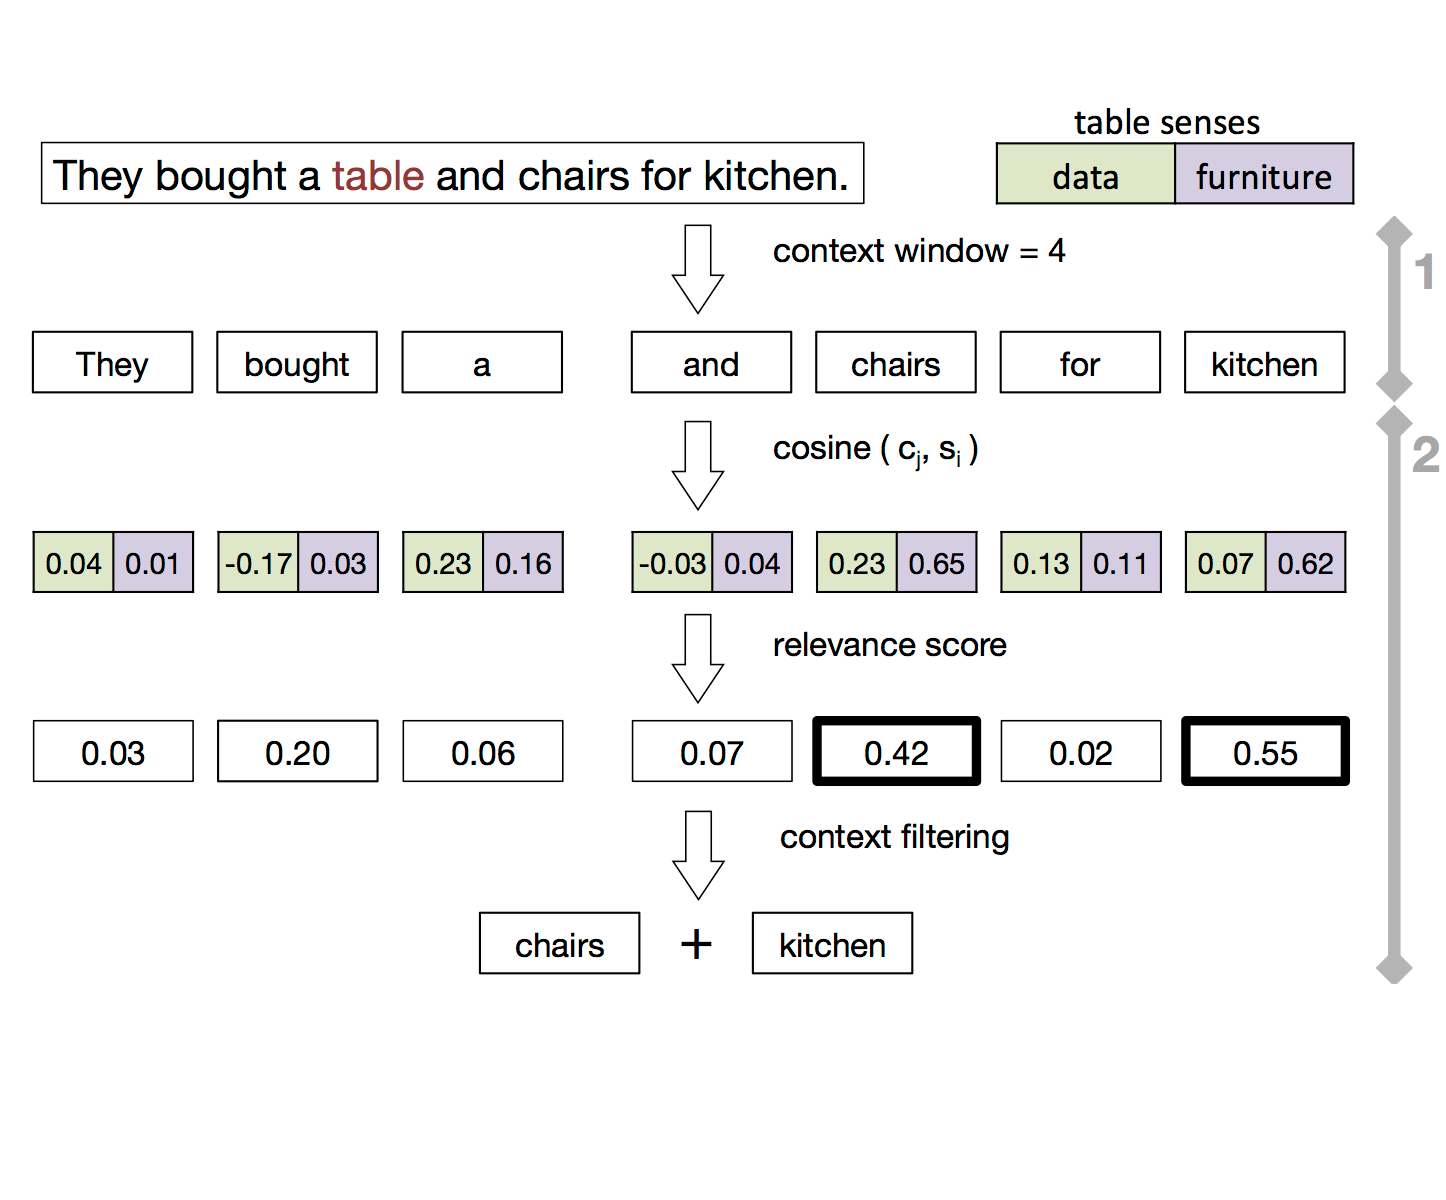
\includegraphics[width=0.82\textwidth]{wsd-3}
\end{center}	
\end{frame}



	
\begin{frame}{Sense embeddings using retrofitting}
%\begin{itemize}
%	\item An example of word sense disambiguation
%\end{itemize}
\vspace{-3em}
	\begin{center}
		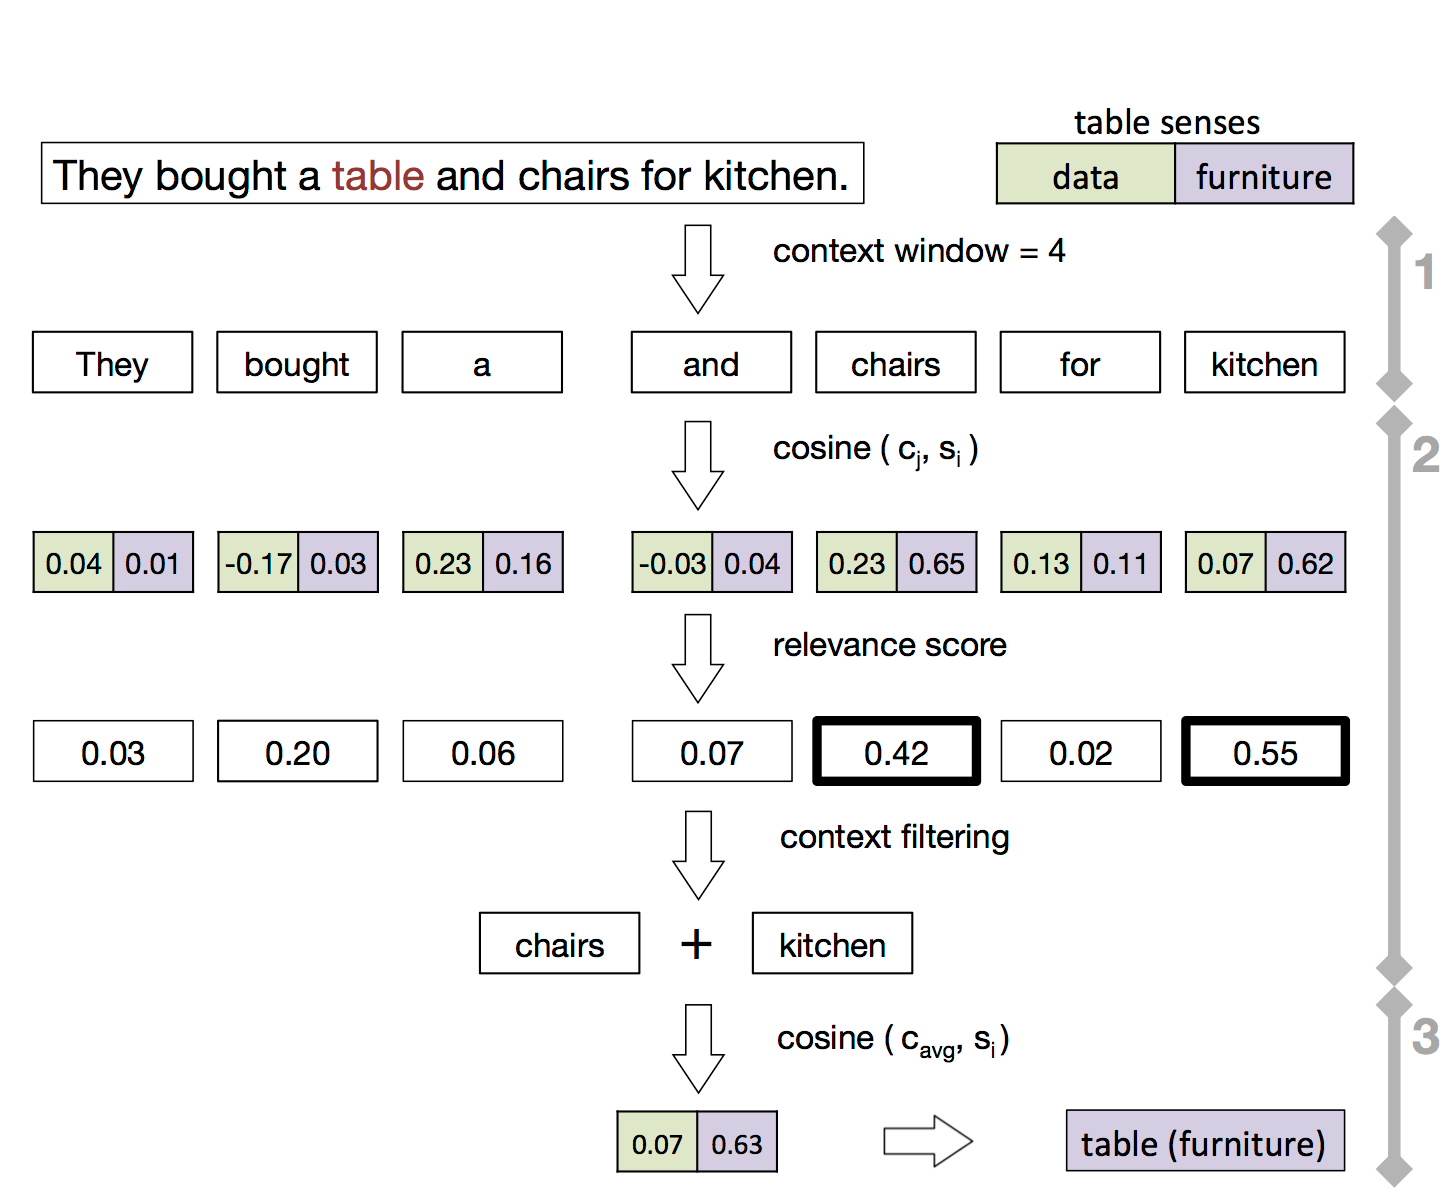
\includegraphics[width=0.82\textwidth]{wsd}
	\end{center}
	
\end{frame}




\begin{frame}{Sense embeddings using retrofitting}

Evaluation on SemEval 2013 Task 13 dataset: comparison to the state-of-the-art

	\vspace{-0.4cm}
	\footnotesize
	\begin{center}
		\begin{tabular}{l|ccc|cc}
			\bf Model & \bf Jacc. & \bf Tau & \bf WNDCG & \bf F.NMI & \bf F.B-Cubed \\ 
			\midrule
			
			AI-KU (add1000) & 0.176 & 0.609 & 0.205 & 0.033 & 0.317 \\
			AI-KU & 0.176 & 0.619 & 0.393 & 0.066 & 0.382 \\
			AI-KU (remove5-add1000) & 0.228 & 0.654 & 0.330 & 0.040 & 0.463 \\
			Unimelb (5p) & 0.198 & 0.623 & 0.374 & 0.056 & 0.475 \\
			Unimelb (50k) & 0.198 & 0.633 & 0.384 & 0.060 & 0.494 \\
			UoS (\#WN senses) & 0.171 & 0.600 & 0.298 & 0.046 & 0.186 \\
			UoS (top-3) & 0.220 & 0.637 & 0.370 & 0.044 & 0.451 \\
			La Sapienza (1) & 0.131 & 0.544 & 0.332 & --  & -- \\
			La Sapienza (2) & 0.131 & 0.535 & 0.394 & -- & -- \\ \midrule
			AdaGram, $\alpha$ = 0.05, 100 dim & 0.274 & 0.644  & 0.318  & 0.058  & 0.470  \\ \midrule
			\alert{w2v}  & 0.197 & 0.615 & 0.291 & 0.011 & 0.615 \\
			%& \wv   -- weighted -- $$p=2$$ -- filter2 -- sw  & 0.197 & 0.614 & 0.291 & 0.012 & 0.615 \\
			\alert{w2v (nouns)} & 0.179 & 0.626 & 0.304 & 0.011 & 0.623 \\
			
			\alert{JBT} & 0.205 & 0.624 & 0.291 & 0.017 & 0.598\\
			\alert{JBT (nouns)} & 0.198 & 0.643 & 0.310 & 0.031 & 0.595\\
			\alert{TWSI (nouns)} & 0.215 & 0.651 & 0.318 & 0.030 & 0.573 \\ 
				
		\end{tabular}
	\end{center}
\end{frame}



\begin{frame}{Sense embeddings using retrofitting}

Results of Steffen ... or summarize both SemEval'13 

\end{frame}


%%%%%%%%%%%%%%%%%%%%%%%%% 

\begin{frame}{Sparse sense representations}
	
\end{frame}


\begin{frame}{Sparse sense representations}
	
\end{frame}

\begin{frame}{Watset: synset induction}
	
\end{frame}


\begin{frame}{Watset: synset induction}
	
\end{frame}


\begin{frame}{Watset: synset induction}
	
\end{frame}


\begin{frame}{Induction of sense semantic classes}
	
\end{frame}

\begin{frame}{Induction of sense semantic classes}
	
\end{frame}

\begin{frame}{Induction of sense semantic classes}
	
\end{frame}

\section{Making induced senses interpretable}

\section{Conclusion}

\begin{frame}{Summary}

\begin{itemize}
	\item How to \textbf{induce word senses}, \textbf{synsets} and \textbf{semantic classes} from text and synonyms.
    \vspace{1em}
    \pause
    
	\item \textbf{Interpretability can be added} on the top of induced word senses in a model agnostic way. 
	\vspace{1em}
    \pause
	
	\item Hypernymy labels \textbf{improve hypernymy extraction}. 
	\vspace{1em}
	\pause
	
	\item Linking induced word senses to lexical resources:
	\begin{itemize} 
		\item improves \textbf{performance of WSD};
		\item can be used to \textbf{enrich lexical resources} with new senses.
	\end{itemize}
	
	
\end{itemize}


\end{frame}


\begin{frame}{A New Shared Task on WSI\&D}
  
  \begin{itemize}
  \item Participate in an ACL SIGSLAV sponsored shared task on \textbf{word sense induction and disambiguation} for Russian!
  
  
 \end{itemize} 
  
  \begin{block}{A lexical sample task evaluated using the ARI measure }
  \begin{itemize}
  	\item Target word, e.g. ``bank'' (in Russian).
  	\item Contexts where the word occurs.
  	\item You need to group the contexts by senses.
  \end{itemize}
   \end{block}
  
  \pause
  \begin{itemize}
    \item \textbf{More details}: \url{http://russe.nlpub.org/2018/wsi}
  \item You can participate by \textbf{31.01.2018}.
     
  \end{itemize}
  
\end{frame}

\begin{frame}{}
\Huge{Thank you!}
\end{frame}

\bibliography{biblio}
\bibliographystyle{apalike}


\end{document}

